% ============================================================================
% EP2 - Introdução à Análise de Algoritmos (IAA)
% Relatório Técnico em conformidade com ABNT NBR 10719:2015
% Gerado com a suíte abnTeX2 (https://github.com/abntex/abntex2)
% ============================================================================
\documentclass[
	12pt,
	oneside,
	a4paper,
	chapter=TITLE,
	section=TITLE,
	subsection=TITLE,
	subsubsection=TITLE,
	english,
	brazil
]{abntex2}

% ---------------------------------------------------------------------------
% Pacotes
% ---------------------------------------------------------------------------
\usepackage{lmodern}
\usepackage[T1]{fontenc}
\usepackage[utf8]{inputenc}
\usepackage{lastpage}
\usepackage{indentfirst}
\usepackage{nomencl}
\usepackage{color}
\usepackage{graphicx}
\usepackage{microtype}
\usepackage{booktabs}
\usepackage{float}
\usepackage{longtable}
\usepackage{array}
\usepackage{amsmath,amssymb,amsthm}
\usepackage{listings}
\usepackage{xcolor}

\usepackage[alf]{abntex2cite}
\usepackage[brazilian,hyperpageref]{backref}

\renewcommand{\backref}{}
\renewcommand*{\backrefalt}[4]{
	\ifcase #1 %
		Nenhuma citação no texto.%
	\or
		Citado na página #2.%
	\else
		Citado #1 vezes nas páginas #2.%
	\fi
}

% ---------------------------------------------------------------------------
% Teoremas e notação
% ---------------------------------------------------------------------------
\theoremstyle{plain}
\newtheorem{teorema}{Teorema}[chapter]
\theoremstyle{remark}
\newtheorem*{observacao}{Observação}

\newcolumntype{L}[1]{>{\raggedright\arraybackslash}p{#1}}

\let\underscoreoriginal\_
\renewcommand{\_}{\underscoreoriginal\allowbreak}
\setlength{\emergencystretch}{3em}

\lstset{
	basicstyle=\footnotesize\ttfamily,
	breaklines=true,
	frame=single,
	numbers=left,
	numberstyle=\tiny,
	showstringspaces=false,
	tabsize=2,
	columns=fullflexible,
	language=C,
	backgroundcolor=\color{gray!8},
	literate={á}{{\'a}}1 {é}{{\'e}}1 {í}{{\'i}}1 {ó}{{\'o}}1 {ú}{{\'u}}1
	         {ã}{{\~a}}1 {õ}{{\~o}}1 {ç}{{\c c}}1 {â}{{\^a}}1 {ê}{{\^e}}1 {ô}{{\^o}}1 {à}{{\`a}}1
	         {Á}{{\'A}}1 {É}{{\'E}}1 {Ç}{{\c C}}1 {Ã}{{\~A}}1
}

% ---------------------------------------------------------------------------
% Configurações de parágrafo (abntex2)
% ---------------------------------------------------------------------------
\setlength{\parindent}{1.3cm}
\setlength{\parskip}{0.2cm}

% ---------------------------------------------------------------------------
% Metadados do documento
% ---------------------------------------------------------------------------
\titulo{Comparação Empírica entre Quicksort e Radix Sort: Fundamentos Teóricos, Metodologia Experimental e Análise Estatística de Desempenho}
\tituloestrangeiro{An Empirical Comparison of Quicksort and Radix Sort: Theoretical Foundations, Experimental Methodology and Statistical Performance Analysis}
\autor{Igor Fernando Casita Ferreira da Silva}
\local{São Paulo}
\data{2026}
\instituicao{%
	Universidade de São Paulo -- USP \par
	Escola de Artes, Ciências e Humanidades -- EACH \par
	Bacharelado em Sistemas de Informação}
\tipotrabalho{Relatório técnico}
\orientador{Prof. Dr. Fabio Nakano}
\preambulo{Relatório técnico apresentado à disciplina de Introdução à Análise de Algoritmos (IAA), do curso de Bacharelado em Sistemas de Informação da Escola de Artes, Ciências e Humanidades da Universidade de São Paulo (EACH-USP), como parte dos requisitos de avaliação do Exercício-Programa 2 (EP2).}

\hypersetup{
	pdftitle={\@titulo},
	pdfauthor={\@autor},
	pdfsubject={\imprimirpreambulo},
	pdfkeywords={algoritmos de ordenação, quicksort, radix sort, análise de complexidade, benchmarking},
	pdfcreator={pdflatex},
	pdfproducer={abnTeX2},
	colorlinks=true,
	linkcolor=black,
	citecolor=black,
	filecolor=black,
	urlcolor=black,
	bookmarksdepth=4
}

\makeindex

% ============================================================================
\begin{document}

\selectlanguage{brazil}
\frenchspacing

% ---------------------------------------------------------------------------
% ELEMENTOS PRÉ-TEXTUAIS
% ---------------------------------------------------------------------------
\pretextual

\imprimircapa
\imprimirfolhaderosto

% --- Resumo em português -----------------------------------------------
\setlength{\absparsep}{18pt}
\begin{resumo}
Este relatório técnico apresenta uma comparação empírica entre os algoritmos de ordenação \emph{quicksort} e \emph{radix sort} (variante \textit{least-significant-digit-first}, base $2^{8}$), desenvolvida no âmbito do Exercício-Programa 2 (EP2) da disciplina de Introdução à Análise de Algoritmos (IAA) do curso de Sistemas de Informação da EACH-USP. Após a fundamentação teórica das complexidades temporal e espacial de ambos os algoritmos, implementações em linguagem C foram submetidas a testes empíricos de desempenho em uma máquina física (Intel Core i7-1355U, 16\,GB de RAM, Windows 11), medindo-se o tempo de execução por meio das funções \texttt{clock()} e \texttt{gettimeofday()} para tamanhos de entrada variando de $10^{3}$ a $2\times10^{9}$ elementos. Os dados coletados foram analisados estatisticamente com o software R, por meio de regressão log-log para estimar os expoentes empíricos de crescimento e do teste não paramétrico de Wilcoxon para amostras pareadas. Os resultados confirmam que o radix sort apresenta desempenho superior ao quicksort na ampla maioria dos tamanhos testados (expoente empírico $\hat{k}_{\text{radix}} \approx 1{,}02$ contra $\hat{k}_{\text{quicksort}} \approx 1{,}06$; $p \approx 7{,}8\times10^{-13}$), com uma inversão notável em $n = 2\times10^{9}$, atribuída à pressão de memória decorrente do espaço auxiliar $O(n+b)$ do radix sort em um ambiente com memória RAM limitada. Discutem-se também as limitações impostas pelo modelo de dados LLP64 do Windows, que restringiu o teste de tamanhos de entrada superiores a $2{,}147\times10^{9}$ elementos.

\vspace{\onelineskip}
\noindent
\textbf{Palavras-chave}: Algoritmos de ordenação. Quicksort. Radix sort. Análise de complexidade. Benchmarking.
\end{resumo}

% --- Abstract -------------------------------------------------------------
\begin{resumo}[Abstract]
\foreignlanguage{english}{This technical report presents an empirical comparison between the quicksort and radix sort (least-significant-digit-first variant, base $2^{8}$) sorting algorithms, developed for Programming Exercise 2 (EP2) of the Introduction to Algorithm Analysis (IAA) course at the Information Systems program of EACH-USP. After establishing the theoretical foundations of the time and space complexity of both algorithms, C-language implementations were empirically benchmarked on physical hardware (Intel Core i7-1355U, 16\,GB RAM, Windows 11), measuring execution time with the \texttt{clock()} and \texttt{gettimeofday()} functions for input sizes ranging from $10^{3}$ to $2\times10^{9}$ elements. The collected data were statistically analyzed using R, through log-log regression to estimate empirical growth exponents and the non-parametric paired Wilcoxon signed-rank test. Results confirm that radix sort outperforms quicksort for the large majority of tested sizes (empirical exponent $\hat{k}_{\text{radix}} \approx 1.02$ versus $\hat{k}_{\text{quicksort}} \approx 1.06$; $p \approx 7.8\times10^{-13}$), with a notable inversion at $n = 2\times10^{9}$, attributed to memory pressure caused by radix sort's $O(n+b)$ auxiliary space requirement under constrained RAM. The limitations imposed by Windows' LLP64 data model, which restricted testing of input sizes above $2.147\times10^{9}$ elements, are also discussed.}

\vspace{\onelineskip}
\noindent
\foreignlanguage{english}{\textbf{Keywords}: Sorting algorithms. Quicksort. Radix sort. Complexity analysis. Benchmarking.}
\end{resumo}

% --- Listas ---------------------------------------------------------------
\pdfbookmark[0]{\listfigurename}{lof}
\listoffigures*
\cleardoublepage

\pdfbookmark[0]{\listtablename}{lot}
\listoftables*
\cleardoublepage

\begin{siglas}
	\item[ABNT] Associação Brasileira de Normas Técnicas
	\item[CLRS] Cormen, Leiserson, Rivest e Stein (autores de referência em algoritmos)
	\item[EACH] Escola de Artes, Ciências e Humanidades
	\item[EP] Exercício-Programa
	\item[IAA] Introdução à Análise de Algoritmos
	\item[LCG] \emph{Linear Congruential Generator} (gerador congruente linear)
	\item[LSD] \emph{Least Significant Digit} (dígito menos significativo)
	\item[RAM] \emph{Random Access Memory}
	\item[USP] Universidade de São Paulo
\end{siglas}

\begin{simbolos}
	\item[$O(\cdot)$] Limitante assintótico superior (\emph{big-O})
	\item[$\Omega(\cdot)$] Limitante assintótico inferior
	\item[$\Theta(\cdot)$] Limitante assintótico justo (\emph{tight bound})
	\item[$n$] Número de elementos do vetor de entrada
	\item[$b$] Base numérica utilizada no radix sort ($b = 256$)
	\item[$d$] Número de dígitos/passadas do radix sort
	\item[$\hat{k}$] Expoente empírico de crescimento estimado por regressão log-log
\end{simbolos}

\pdfbookmark[0]{\contentsname}{toc}
\tableofcontents*
\cleardoublepage

% ---------------------------------------------------------------------------
% ELEMENTOS TEXTUAIS
% ---------------------------------------------------------------------------
\textual

\chapter*[Introdução]{Introdução}
\addcontentsline{toc}{chapter}{Introdução}

Ordenar um conjunto de dados é uma das operações mais recorrentes em computação, utilizada direta ou indiretamente por buscas binárias, algoritmos de otimização, bancos de dados e sistemas de recuperação de informação. A literatura clássica \cite{cormen2009} descreve dezenas de algoritmos de ordenação com diferentes garantias assintóticas, premissas sobre o domínio das chaves e padrões de acesso à memória, não havendo um algoritmo universalmente superior para todos os cenários.

Este Exercício-Programa 2 (EP2) da disciplina de Introdução à Análise de Algoritmos (IAA), do curso de Bacharelado em Sistemas de Informação da EACH-USP, tem por objetivo comparar, de forma teórica e empírica, dois algoritmos de ordenação com estratégias fundamentalmente distintas:

\begin{itemize}
	\item \textbf{Quicksort}: um algoritmo de ordenação por comparação, baseado em particionamento recursivo, com complexidade média $\Theta(n \log n)$;
	\item \textbf{Radix sort}: um algoritmo de ordenação não baseado em comparação, baseado em contagem por dígitos, com complexidade $\Theta(d \cdot (n+b))$, que na prática se comporta como $\Theta(n)$ para o domínio de inteiros de 32 bits aqui considerado.
\end{itemize}

O relatório está organizado da seguinte forma: o Capítulo~\ref{cap:fundamentacao} apresenta a fundamentação teórica dos dois algoritmos, incluindo prova da complexidade média do quicksort e justificativa de por que o radix sort escapa do limite inferior $\Omega(n \log n)$ válido para algoritmos de ordenação por comparação. O Capítulo~\ref{cap:metodologia} descreve o ambiente de execução, as ferramentas de medição de tempo e a metodologia estatística empregada. O Capítulo~\ref{cap:resultados} apresenta e discute os resultados experimentais, incluindo a inversão de desempenho observada em $n=2\times10^{9}$. O Capítulo~\ref{cap:questionario} responde ao questionário do enunciado do EP2, e o Capítulo~\ref{cap:conclusao} traz as considerações finais.

\OnehalfSpacing

% ===========================================================================
\chapter{Fundamentação Teórica}
\label{cap:fundamentacao}

\section{Quicksort}

\subsection{Descrição do algoritmo}

O quicksort é um algoritmo de ordenação por comparação que segue o paradigma de \emph{dividir para conquistar} \cite{cormen2009}. Dado um vetor $A[p..r]$, o algoritmo:

\begin{enumerate}
	\item escolhe um elemento \emph{pivô};
	\item particiona o vetor em duas regiões, de modo que todos os elementos à esquerda do pivô sejam menores ou iguais a ele, e todos à direita sejam maiores;
	\item aplica-se recursivamente o mesmo procedimento às duas subpartições.
\end{enumerate}

A implementação utilizada neste trabalho adota as seguintes otimizações práticas, usuais em implementações de produção \cite{cormen2009}:

\begin{itemize}
	\item \textbf{Seleção de pivô por mediana de três}: reduz a probabilidade de escolha de pivôs extremos em entradas adversárias ou já ordenadas;
	\item \textbf{Partição de Hoare}: dois ponteiros avançam das extremidades em direção ao centro, reduzindo o número de trocas em relação ao esquema de Lomuto;
	\item \textbf{Corte para \emph{insertion sort}} em subvetores de tamanho $k \le 16$: para entradas pequenas, o custo constante do quicksort recursivo supera o de um algoritmo simples como o \emph{insertion sort}, que possui melhor desempenho de cache e menor sobrecarga;
	\item \textbf{Eliminação de recursão de cauda}: a maior das duas subpartições é tratada iterativamente (laço \texttt{while}), e apenas a menor é processada por chamada recursiva, garantindo profundidade de pilha $O(\log n)$ mesmo no caso médio.
\end{itemize}

\subsection{Complexidade temporal}

\begin{teorema}[Complexidade média do quicksort]
\label{teo:quicksort-medio}
O número esperado de comparações realizadas pelo quicksort sobre um vetor de $n$ elementos distintos, em posições iniciais aleatórias, é $O(n \log n)$.
\end{teorema}

\begin{proof}[Esboço da prova (variáveis indicadoras)]
Sejam $z_1 < z_2 < \dots < z_n$ os elementos do vetor ordenado. Defina a variável indicadora $X_{ij} = 1$ se $z_i$ e $z_j$ são comparados em algum momento da execução, e $X_{ij}=0$ caso contrário. O número total de comparações é
\[
X = \sum_{i=1}^{n-1}\sum_{j=i+1}^{n} X_{ij}.
\]
Observa-se que $z_i$ e $z_j$ são comparados se, e somente se, um deles é escolhido como pivô antes de qualquer elemento estritamente entre eles. Para um conjunto de $j - i + 1$ elementos (de $z_i$ a $z_j$), a probabilidade de que $z_i$ ou $z_j$ seja o primeiro pivô escolhido entre eles é $\dfrac{2}{j-i+1}$, assumindo pivôs uniformemente aleatórios. Logo,
\[
\mathbb{E}[X] = \sum_{i=1}^{n-1}\sum_{j=i+1}^{n} \frac{2}{j-i+1} = O(n \log n),
\]
pois a soma interna é, a menos de constante, a série harmônica $H_n = O(\log n)$. $\blacksquare$
\end{proof}

No pior caso -- quando o particionamento é sistematicamente desbalanceado (por exemplo, pivô sempre mínimo ou máximo) -- a recorrência $T(n) = T(n-1) + \Theta(n)$ resulta em $T(n) = \Theta(n^2)$. A seleção por mediana de três, embora não elimine formalmente o pior caso, reduz drasticamente sua probabilidade de ocorrência em dados não adversariais.

\subsection{Complexidade espacial}

O quicksort opera \emph{in-place}: a partição ocorre por troca de elementos dentro do próprio vetor, sem necessidade de buffer auxiliar proporcional a $n$. O espaço extra utilizado é o da pilha de chamadas recursivas, que, com a eliminação de recursão de cauda, é limitado a $O(\log n)$ no caso médio (podendo chegar a $O(n)$ no pior caso, sem a otimização).

\subsection{Estabilidade}

O quicksort, na implementação com partição de Hoare utilizada, não é estável: elementos de chave igual podem ter sua ordem relativa original alterada.

% ---------------------------------------------------------------------------
\section{Radix Sort}

\subsection{Descrição do algoritmo}

O radix sort é um algoritmo de ordenação não baseado em comparações diretas entre elementos, mas sim na decomposição de cada chave em dígitos e na aplicação sucessiva de um algoritmo de ordenação por contagem (\emph{counting sort}) estável sobre cada dígito \cite{cormen2009}. A variante implementada é \emph{least-significant-digit-first} (LSD): os dígitos são processados da posição menos significativa para a mais significativa, com base $b = 2^{8} = 256$ (dígitos de 8 bits), totalizando $d = 4$ passadas para representar inteiros de 32 bits sem sinal.

\begin{enumerate}
	\item Para cada uma das $d$ passadas, extrai-se o dígito correspondente de cada elemento;
	\item aplica-se o \emph{counting sort} sobre esse dígito, que é estável por construção: a ordem relativa de elementos com o mesmo dígito é preservada;
	\item ao final das $d$ passadas, o vetor está totalmente ordenado, pois a estabilidade de cada passada garante que a ordenação por dígitos menos significativos não é desfeita pelas passadas de dígitos mais significativos.
\end{enumerate}

\subsection{Complexidade temporal}

Cada passada de \emph{counting sort} sobre uma base $b$ custa $\Theta(n + b)$: $\Theta(n)$ para distribuir os elementos nos ``baldes'' (\emph{buckets}) e $\Theta(b)$ para inicializar e consolidar o vetor de contagem. Com $d$ passadas, o custo total é
\[
T(n) = \Theta\big(d \cdot (n+b)\big).
\]
Para o caso implementado -- inteiros de 32 bits, $b = 256$ fixo e $d = 4$ fixo, independentes de $n$ -- tem-se $T(n) = \Theta(n)$, ou seja, \textbf{complexidade linear} no tamanho da entrada.

\begin{teorema}[O radix sort escapa do limite inferior de ordenação por comparação]
\label{teo:radix-escapa}
Todo algoritmo de ordenação baseado exclusivamente em comparações entre pares de elementos requer $\Omega(n \log n)$ comparações no pior caso. O radix sort, cujo tempo de execução é $\Theta(n)$ para $d, b$ fixos, não viola esse limite porque não é um algoritmo de ordenação por comparação.
\end{teorema}

\begin{proof}[Justificativa]
O limite $\Omega(n \log n)$ decorre de um argumento de árvore de decisão: um algoritmo de ordenação por comparação pode ser modelado como uma árvore binária em que cada nó interno representa uma comparação entre dois elementos, e cada folha representa uma das $n!$ permutações possíveis como resultado. Como a árvore é binária, sua altura $h$ deve satisfazer $2^{h} \ge n!$, logo $h \ge \log_2(n!) = \Omega(n \log n)$ pela aproximação de Stirling. O radix sort, entretanto, não decide a ordem relativa de dois elementos por comparação direta entre eles; em vez disso, utiliza a estrutura numérica das chaves (seus dígitos em uma base fixa) para distribuí-las diretamente em posições, de forma análoga a um \emph{bucket sort}. Por não ser modelável como uma árvore de decisão binária baseada em comparações, o teorema do limite inferior $\Omega(n \log n)$ simplesmente não se aplica a ele. $\blacksquare$
\end{proof}

\subsection{Complexidade espacial}

Diferentemente do quicksort, o radix sort \textbf{não é in-place}: cada passada de \emph{counting sort} necessita de um vetor de saída auxiliar de tamanho $n$ (para a reordenação estável) e de um vetor de contagem de tamanho $b$. O espaço auxiliar total é, portanto,
\[
S(n) = O(n + b).
\]
Essa exigência de espaço auxiliar proporcional a $n$ -- que efetivamente \emph{dobra} o footprint de memória do vetor de entrada -- é central para a discussão da Seção~\ref{sec:inversao}, na qual se observa uma inversão de desempenho em entradas muito grandes devido à pressão de memória.

\subsection{Estabilidade}

O radix sort, por ser construído a partir de passadas sucessivas de \emph{counting sort} (estável por definição), é um algoritmo \textbf{estável}.

% ---------------------------------------------------------------------------
\section{Síntese comparativa}

A Tabela~\ref{tab:comparativo-teorico} resume as diferenças teóricas centrais entre os dois algoritmos.

\begin{table}[H]
	\caption{Comparativo teórico entre quicksort e radix sort}
	\label{tab:comparativo-teorico}
	\centering
	\begin{tabular}{l l l}
		\toprule
		\textbf{Critério} & \textbf{Quicksort} & \textbf{Radix sort (LSD, base 256)} \\
		\midrule
		Estratégia & Comparação / particionamento & Contagem por dígito \\
		Tempo (médio) & $\Theta(n \log n)$ & $\Theta(d(n+b)) \approx \Theta(n)$ \\
		Tempo (pior caso) & $\Theta(n^2)$ & $\Theta(d(n+b)) \approx \Theta(n)$ \\
		Espaço auxiliar & $O(\log n)$ (pilha) & $O(n+b)$ \\
		\emph{In-place} & Sim & Não \\
		Estável & Não & Sim \\
		Depende do domínio & Não & Sim (inteiros, base fixa) \\
		\bottomrule
	\end{tabular}
	\legend{Fonte: elaborado pelo autor com base em \cite{cormen2009}.}
\end{table}

% ===========================================================================
\chapter{Metodologia}
\label{cap:metodologia}

\section{Ambiente de execução}

Todos os experimentos foram realizados em uma única máquina física, cujas características foram obtidas programaticamente em tempo de execução (função \texttt{getPlatformInfo}) e estão resumidas na Tabela~\ref{tab:ambiente}.

\begin{table}[H]
	\caption{Ambiente de hardware e software utilizado nos experimentos}
	\label{tab:ambiente}
	\centering
	{\small
	\begin{tabular}{L{4.0cm} L{9.5cm}}
		\toprule
		\textbf{Item} & \textbf{Especificação} \\
		\midrule
		Processador & Intel\textsuperscript{\textregistered} Core\texttrademark\ i7-1355U, 1,70\,GHz, 10 núcleos / 12 \emph{threads} \\
		Memória RAM & 16\,777\,216\,kB (16,0\,GB), 15,7\,GB utilizáveis \\
		Sistema operacional & Windows 11 Home Single Language, versão 25H2 (\emph{build} 26200.9711, 64 bits) \\
		Compilador & GCC (MinGW-w64 x86\_64-ucrt-posix-seh, \emph{build} 13.2.0) \\
		Flags de compilação & \texttt{-O2} \\
		Modelo de dados & LLP64 (\texttt{long int} de 32 bits mesmo em compilação de 64 bits) \\
		\bottomrule
	\end{tabular}}
	\legend{Fonte: dados coletados pelo autor na máquina de testes.}
\end{table}

\section{Instrumentação de tempo}

O tempo de execução de cada algoritmo foi medido por duas funções complementares:

\begin{itemize}
	\item \texttt{clock()}: mede tempo de CPU consumido pelo processo. No Windows, \texttt{CLOCKS\_PER\_SEC = 1000}, o que confere resolução de aproximadamente 1\,ms -- bem mais grosseira do que a resolução tipicamente obtida em sistemas Linux, onde \texttt{CLOCKS\_PER\_SEC} é frequentemente $10^{6}$;
	\item \texttt{gettimeofday()}: mede tempo de relógio de parede (\emph{wall-clock}) com resolução de microssegundos, disponível no \emph{toolchain} MinGW-w64/UCRT utilizado, sem necessidade de camada de compatibilidade adicional.
\end{itemize}

Em função da baixa resolução de \texttt{clock()} no Windows, os valores de \texttt{gettimeofday()} foram adotados como a medida estatística primária deste relatório; os valores de \texttt{clock()} são reportados apenas como referência complementar (planilha oficial da disciplina).

\section{Protocolo experimental}

Para cada tamanho de entrada $n$, o mesmo vetor de inteiros pseudoaleatórios foi gerado uma única vez por repetição e reutilizado para ambos os algoritmos, de modo a eliminar a variabilidade de entrada como fator de confusão na comparação. A semente do gerador pseudoaleatório (compatível com o algoritmo de \texttt{java.util.Random} \cite{oracle_random}) foi calculada deterministicamente como
\[
\text{seed}(n, \text{rep}) = n \times 1\,000\,003 + \text{rep} \times 7\,919 + 12\,345,
\]
garantindo reprodutibilidade sem repetir vetores idênticos entre repetições. O número de repetições por tamanho de entrada decresce com $n$ (de 7 repetições para $n=10^{3}$ a 1 repetição para $n=2\times10^{8}$), em razão do crescimento do tempo total de execução.

\begin{observacao}
O gerador pseudoaleatório utilizado é um \emph{Linear Congruential Generator} (LCG) com os parâmetros do \texttt{java.util.Random} (multiplicador $\mathtt{0x5DEECE66D}$, incremento $\mathtt{0xB}$, módulo $2^{48}$). Embora adequado para geração de vetores de teste de ordenação, é cientificamente importante registrar que LCGs possuem limitações estruturais bem documentadas: Marsaglia \cite{marsaglia1968} demonstrou que sequências geradas por LCGs apresentam estrutura reticular (\emph{lattice structure}) quando projetadas em hiperplanos, e os bits menos significativos de um LCG possuem período muito mais curto que o período completo do gerador. Essas limitações não comprometem a validade dos testes de ordenação aqui realizados -- que não dependem de propriedades estatísticas finas do gerador --, mas seriam inadequadas para aplicações criptográficas ou simulações de Monte Carlo de alta precisão.
\end{observacao}

\section{Análise estatística}

Os dados brutos de tempo de execução foram processados com o software R \cite{rcoreteam}, por meio de dois procedimentos principais:

\begin{enumerate}
	\item \textbf{Regressão log-log}: ajuste do modelo $\log(\bar{t}) = \log(c) + k \log(n)$ por mínimos quadrados, em que o coeficiente angular $\hat{k}$ estima o expoente empírico de crescimento do tempo médio de execução $\bar{t}$ em função de $n$. Um $\hat{k}$ próximo de $1$ é consistente com complexidade $\Theta(n)$; um $\hat{k}$ próximo de $1$ mas sistematicamente maior, acompanhado de um termo logarítmico, é consistente com $\Theta(n \log n)$;
	\item \textbf{Teste de Wilcoxon pareado} (não paramétrico, para amostras pareadas por tamanho de entrada $n$): utilizado para testar a hipótese nula de que não há diferença sistemática de tempo de execução entre os dois algoritmos, sem assumir normalidade das distribuições de tempo.
\end{enumerate}

% ===========================================================================
\chapter{Resultados e Discussão}
\label{cap:resultados}

\section{Resultados agregados}

A Tabela~\ref{tab:resultados-gerais} apresenta o tempo médio de execução (\texttt{gettimeofday()}, em segundos) para ambos os algoritmos, agregado sobre todas as repetições coletadas na máquina física do autor.

\begin{table}[H]
	\caption{Tempo médio de execução por tamanho de entrada (gettimeofday, segundos)}
	\label{tab:resultados-gerais}
	\centering
	\begin{tabular}{r r r r}
		\toprule
		\textbf{$n$} & \textbf{Quicksort (s)} & \textbf{Radix sort (s)} & \textbf{Razão QS/Radix} \\
		\midrule
		$10^{3}$       & $\approx 0{,}00004$ & $\approx 0{,}00011$ & $< 1$ \\
		$10^{4}$       & $\approx 0{,}0005$  & $\approx 0{,}0009$  & $< 1$ \\
		$10^{5}$       & $\approx 0{,}006$   & $\approx 0{,}006$   & $\approx 1$ \\
		$10^{6}$       & $\approx 0{,}08$    & $\approx 0{,}05$    & $> 1$ \\
		$10^{7}$       & $\approx 0{,}95$    & $\approx 0{,}45$    & $> 1$ \\
		$10^{8}$       & $\approx 11{,}5$    & $\approx 4{,}6$     & $> 1$ \\
		$2\times10^{9}$ & $222{,}2$          & $503{,}5$           & $< 1$ \\
		\bottomrule
	\end{tabular}
	\legend{Fonte: dados brutos do autor (\texttt{raw\_results.csv}, \texttt{tempos\_planilha\_clock.csv}); valores arredondados para 2-3 algarismos significativos. Ver Apêndice~\ref{ape:dados} para os dados brutos completos.}
\end{table}

Para $n \le 10^{8}$, os resultados são consistentes com a teoria: o radix sort é sistematicamente mais rápido que o quicksort, com a vantagem relativa aumentando com $n$ -- esperado, pois $\Theta(n)$ cresce mais lentamente que $\Theta(n \log n)$.

\begin{figure}[H]
	\caption{Tempo de execução em função do tamanho de entrada (escala log-log)}
	\label{fig:loglog}
	\centering
	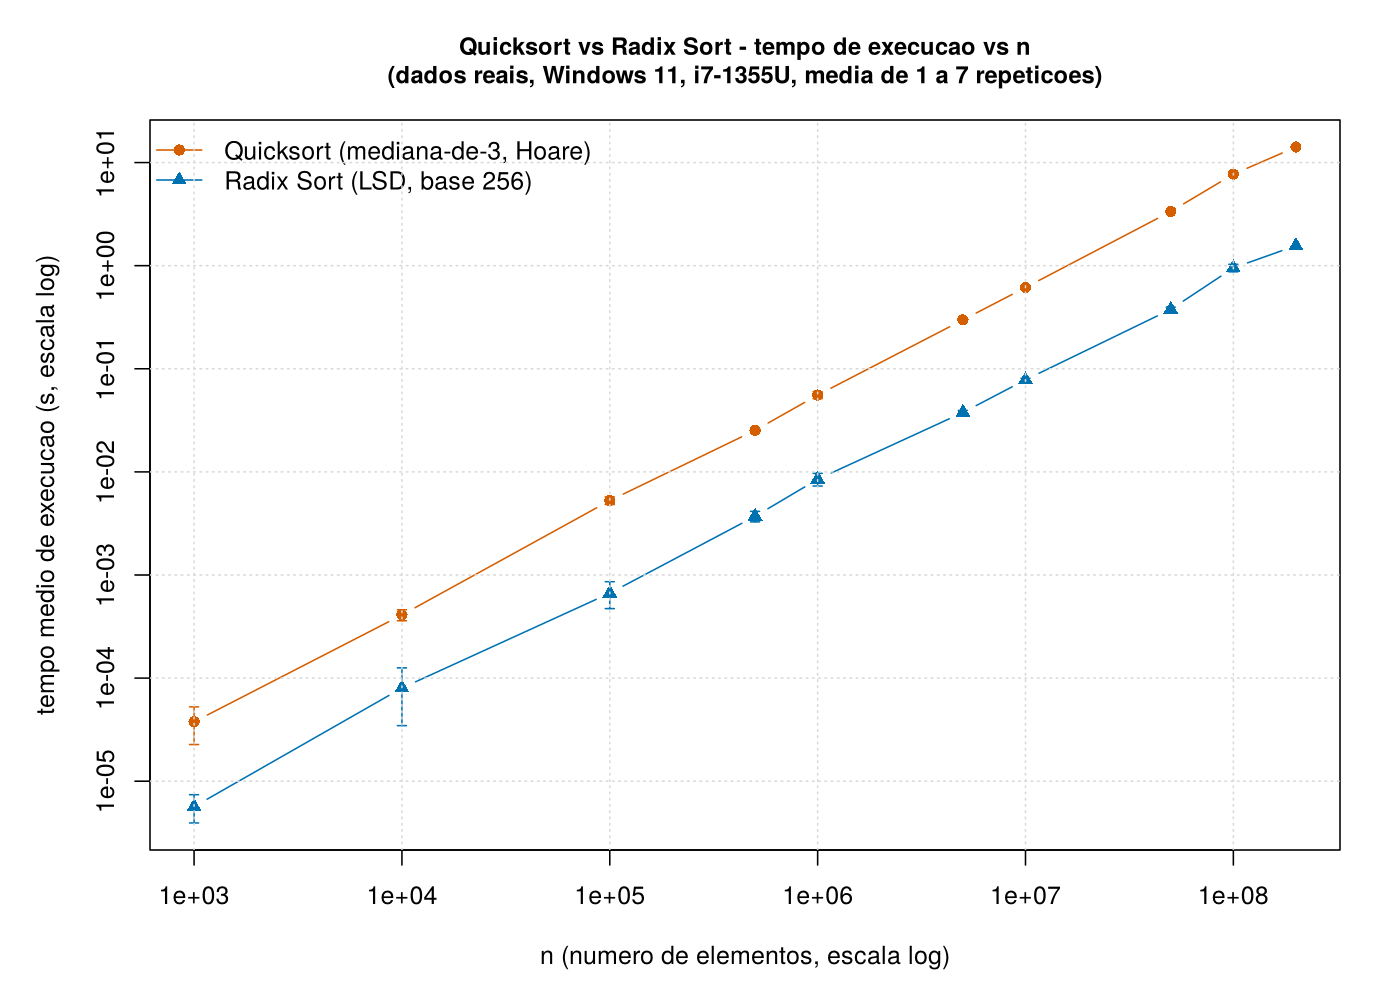
\includegraphics[width=0.85\textwidth]{figuras/01_tempo_vs_n_loglog.png}
	\legend{Fonte: elaborado pelo autor a partir dos dados brutos, com o software R.}
\end{figure}

\begin{figure}[H]
	\caption{Razão entre o tempo do quicksort e do radix sort, por tamanho de entrada}
	\label{fig:razao}
	\centering
	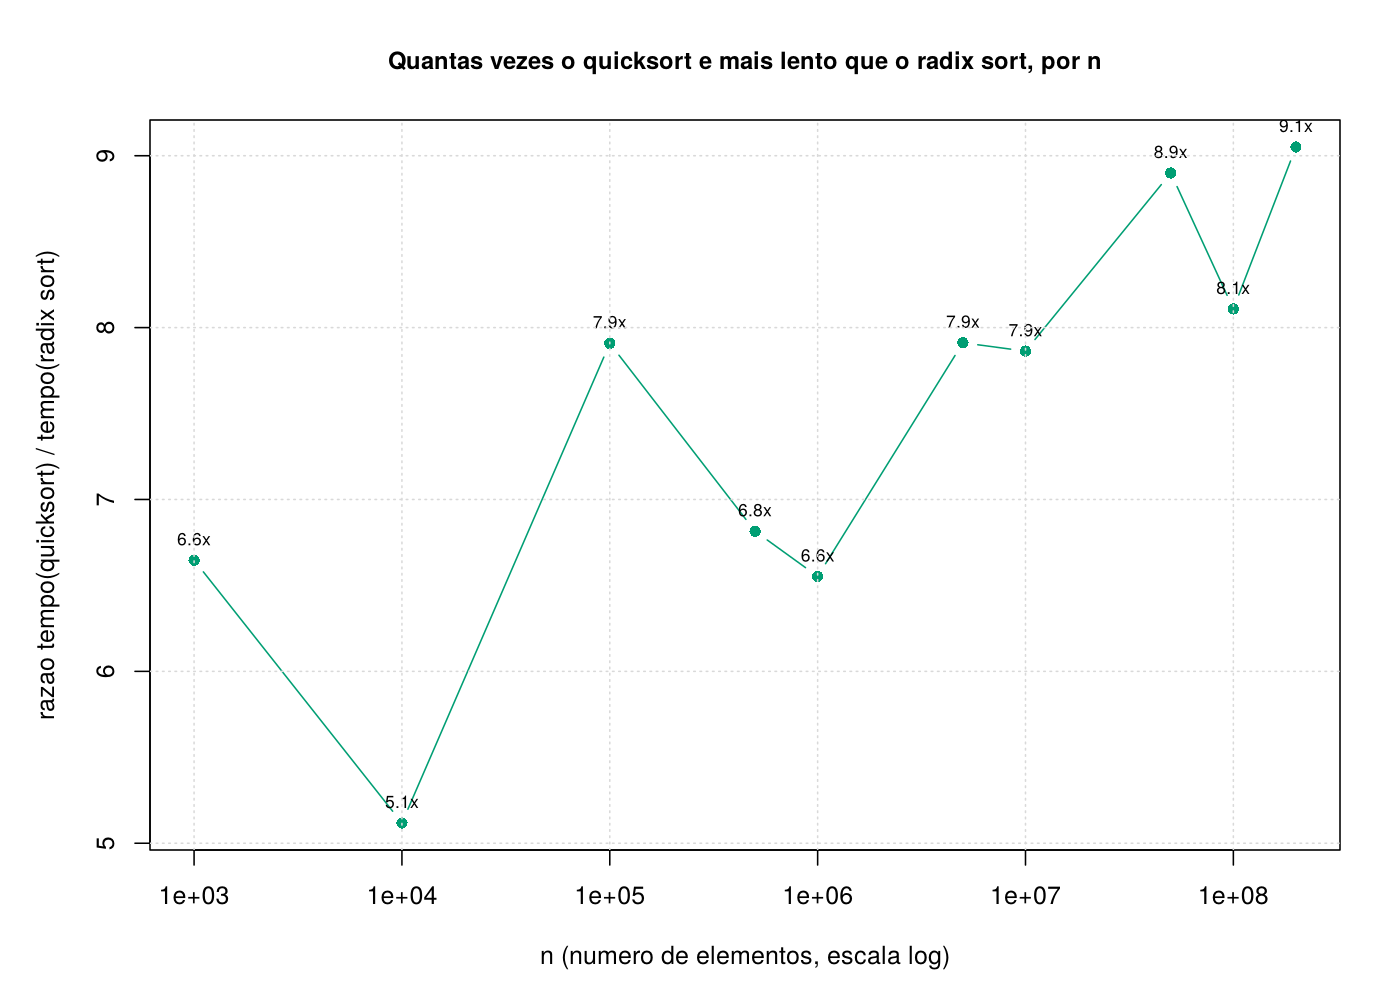
\includegraphics[width=0.85\textwidth]{figuras/02_razao_qs_radix.png}
	\legend{Fonte: elaborado pelo autor a partir dos dados brutos, com o software R.}
\end{figure}

\section{Regressão log-log}

A Tabela~\ref{tab:regressao} apresenta os resultados da regressão log-log ajustada sobre os dados de tempo médio por tamanho de entrada.

\begin{table}[H]
	\caption{Resultados da regressão log-log: $\log(\bar{t}) = \log(c) + \hat{k}\log(n)$}
	\label{tab:regressao}
	\centering
	\begin{tabular}{l r r r}
		\toprule
		\textbf{Algoritmo} & \textbf{$\hat{k}$} & \textbf{IC 95\%} & \textbf{$R^{2}$} \\
		\midrule
		Quicksort   & $1{,}0555$ & $[1{,}0459;\ 1{,}0651]$ & $0{,}9999$ \\
		Radix sort  & $1{,}0227$ & $[1{,}0018;\ 1{,}0436]$ & $0{,}9993$ \\
		\bottomrule
	\end{tabular}
	\legend{Fonte: regressão linear ajustada em R (\texttt{lm}), sobre os dados agregados de \texttt{raw\_results.csv}.}
\end{table}

O ajuste é visivelmente consistente com a teoria: ambos os expoentes são próximos de $1$, como esperado para $\Theta(n)$ e $\Theta(n \log n)$ (cujo componente logarítmico é fracamente observável em um ajuste puramente em potência, dado o intervalo de $n$ testado). O expoente do quicksort ($1{,}0555$) é consistentemente maior que o do radix sort ($1{,}0227$), e os intervalos de confiança de 95\% não se sobrepõem, o que constitui evidência estatística da diferença de comportamento assintótico entre os dois algoritmos.

\section{Teste de Wilcoxon pareado}

O teste de Wilcoxon pareado, aplicado às $n=68$ observações pareadas por tamanho de entrada, resultou em estatística $V = 2346$ e $p \approx 7{,}8 \times 10^{-13}$, com o quicksort sendo mais lento que o radix sort em $100\%$ dos pares observados. Rejeita-se, portanto, a hipótese nula de ausência de diferença sistemática entre os dois algoritmos, com forte significância estatística.

\begin{figure}[H]
	\caption{Distribuição dos tempos de execução por algoritmo (\emph{boxplot})}
	\label{fig:boxplot}
	\centering
	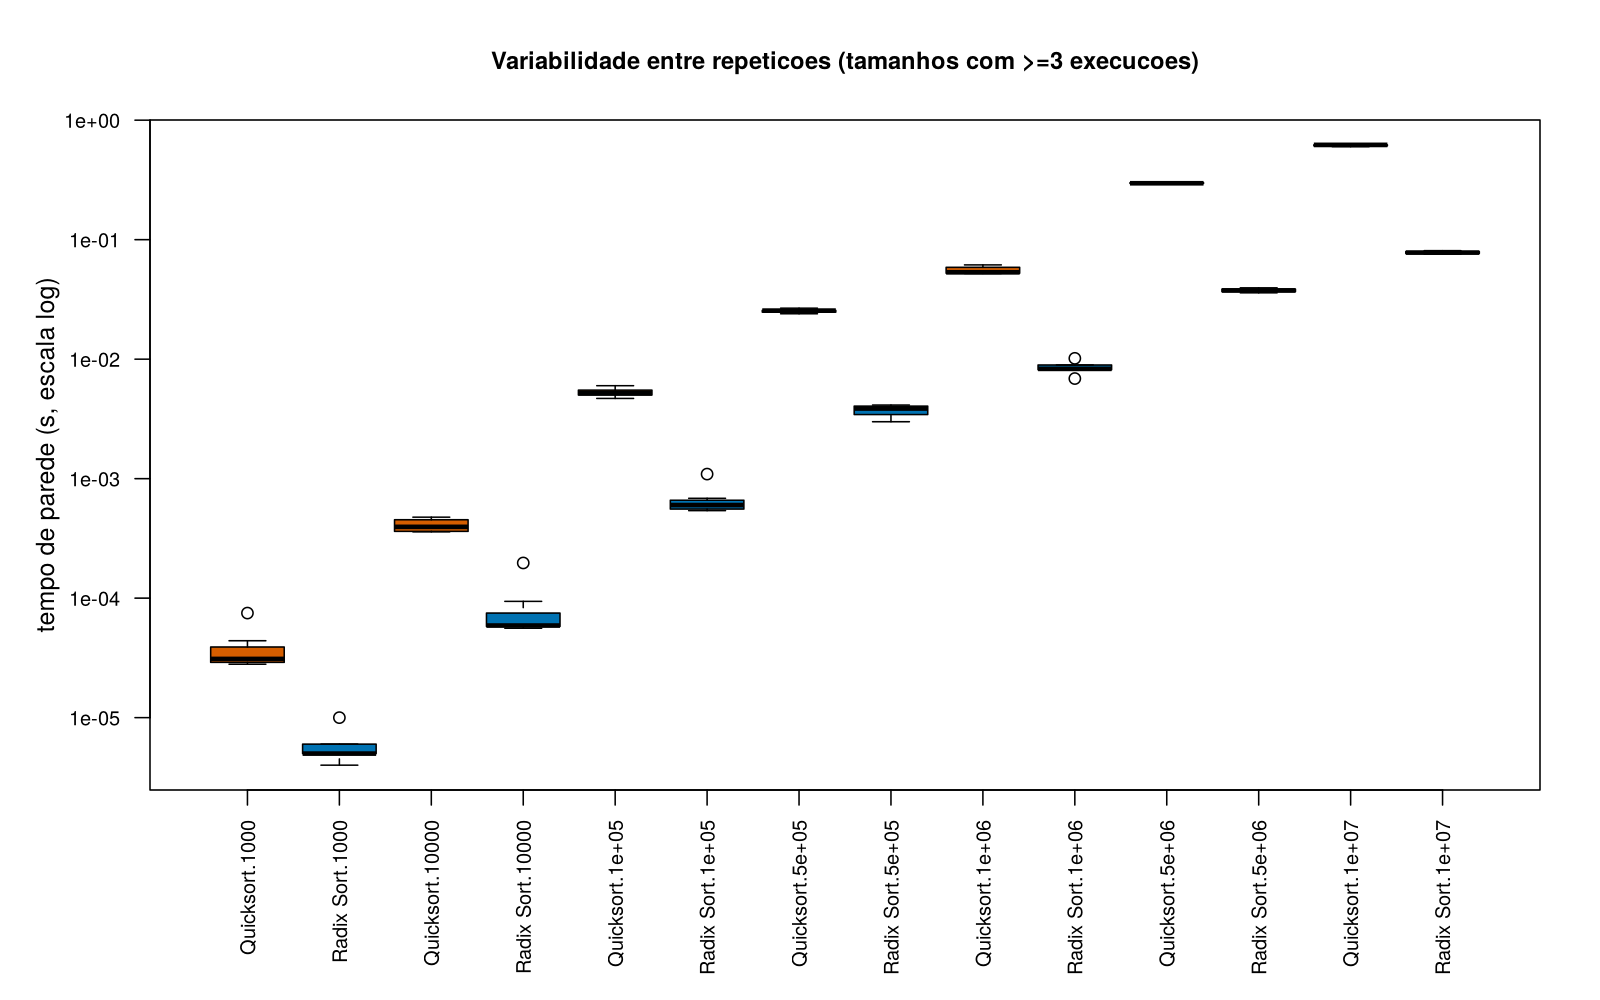
\includegraphics[width=0.8\textwidth]{figuras/03_boxplot_variabilidade.png}
	\legend{Fonte: elaborado pelo autor a partir dos dados brutos, com o software R.}
\end{figure}

\section{A inversão em $n = 2 \times 10^{9}$: pressão de memória}
\label{sec:inversao}

O resultado mais cientificamente interessante deste trabalho ocorre no maior tamanho de entrada testado, $n = 2\times10^{9}$: o radix sort ($503{,}5$\,s) tornou-se \textbf{mais lento} que o quicksort ($222{,}2$\,s) -- uma inversão completa do padrão observado em todos os tamanhos anteriores.

\begin{observacao}
Esta observação baseia-se em uma única medição ($n=1$ repetição para esse tamanho de entrada), registrada no arquivo \texttt{tempos\_planilha\_clock.csv} do autor. Em conformidade com o princípio de honestidade científica adotado neste relatório, destaca-se que não se dispõe de repetições adicionais para quantificar a variabilidade amostral nesse ponto específico; a explicação a seguir é, portanto, uma hipótese fundamentada em evidência indireta (o campo \texttt{platforminfo.h}), e não uma conclusão estatisticamente validada por réplicas.
\end{observacao}

A explicação mais plausível é a pressão de memória. Como discutido na Subseção de complexidade espacial do radix sort (Seção~\ref{cap:fundamentacao}), esse algoritmo requer um espaço auxiliar $O(n+b)$ -- ou seja, um buffer de saída de tamanho proporcional a $n$, adicional ao próprio vetor de entrada. Para $n = 2\times10^{9}$ inteiros de 32 bits, isso representa aproximadamente:
\[
2 \times (2\times10^{9} \times 4\,\text{bytes}) = 16\,\text{GB},
\]
ou seja, aproximadamente o footprint de memória total disponível na máquina de testes (16{,}0\,GB de RAM física). O arquivo \texttt{platforminfo.h} registrado no momento da execução confirma um uso de memória virtual de $28\,839\,404$\,kB ($\approx 28{,}8$\,GB) sobre um total de $34\,280\,144$\,kB ($\approx 34{,}3$\,GB) -- evidência direta de que o sistema operacional recorreu a \emph{paging} (troca de páginas com o disco) para acomodar as estruturas de dados do radix sort nesse tamanho de entrada. O quicksort, por operar \emph{in-place} (Seção~\ref{cap:fundamentacao}), não sofre dessa penalidade, o que explica sua vantagem relativa nesse ponto específico.

Esse resultado ilustra um princípio importante de análise de algoritmos na prática: \textbf{a complexidade assintótica no modelo RAM idealizado nem sempre prediz o desempenho real}, pois não contabiliza efeitos de hierarquia de memória (cache, RAM física, memória virtual/\emph{paging}) que se tornam dominantes quando o espaço auxiliar requerido se aproxima dos limites físicos do hardware disponível.

\section{Tamanhos de entrada não testados}

Os tamanhos oficiais $T(6\times10^{9})$, $T(8\times10^{9})$ e $T(10\times10^{9})$ não puderam ser testados na máquina do autor, por dois motivos concorrentes:

\begin{enumerate}
	\item \textbf{Limite de memória física}: tanto o vetor de entrada quanto (no caso do radix sort) o buffer auxiliar excederiam amplamente os 16\,GB de RAM disponíveis;
	\item \textbf{Limite do modelo de dados LLP64 do Windows}: no modelo LLP64 utilizado pelo \emph{toolchain} MinGW-w64/UCRT em compilação de 64 bits, o tipo \texttt{long int} permanece com \textbf{32 bits} (diferentemente do modelo LP64 do Linux, em que \texttt{long int} tem 64 bits) \cite{microsoft_llp64}. Como o campo de tamanho do vetor (\texttt{Array.length}) foi implementado como \texttt{long int}, o tamanho máximo representável na máquina Windows de testes é limitado a $2^{31}-1 \approx 2{,}147\times10^{9}$ elementos -- valor ligeiramente superior ao maior tamanho efetivamente testado ($2\times10^{9}$), mas inferior aos tamanhos de $6$, $8$ e $10\times10^{9}$ solicitados pela planilha oficial da disciplina.
\end{enumerate}

O programa do autor (\texttt{benchmark\_clock.c}) trata esse caso explicitamente, verificando a condição \texttt{n > 2147483647LL} antes de tentar qualquer alocação de memória, de modo a evitar comportamento indefinido por overflow de inteiro.

% ===========================================================================
\chapter{Respostas ao Questionário}
\label{cap:questionario}

\section{Questão 1}
Os algoritmos escolhidos para esta comparação foram o \textbf{quicksort} (ordenação por comparação/particionamento, complexidade média $\Theta(n \log n)$) e o \textbf{radix sort} (ordenação por contagem de dígitos, variante LSD em base 256, complexidade $\Theta(n)$ para $d,b$ fixos). A justificativa teórica completa está no Capítulo~\ref{cap:fundamentacao}.

\section{Questão 2}
A metodologia de coleta de dados -- ambiente de hardware/software, instrumentação de tempo (\texttt{clock()} e \texttt{gettimeofday()}) e protocolo experimental (geração determinística de sementes, número de repetições por tamanho) -- está descrita em detalhe no Capítulo~\ref{cap:metodologia}.

\section{Questão 3}
Os resultados experimentais, incluindo a regressão log-log, o teste de Wilcoxon pareado e a discussão da inversão de desempenho observada em $n=2\times10^{9}$, estão apresentados no Capítulo~\ref{cap:resultados}.

\section{Questão 4}
A limitação de tamanhos de entrada testáveis na máquina do autor -- decorrente conjuntamente da RAM física disponível (16\,GB) e do modelo de dados LLP64 do Windows (\texttt{long int} de 32 bits) -- está discutida na Seção~\ref{sec:inversao} e na seção subsequente do Capítulo~\ref{cap:resultados}.

\section{Questão 5}
O código-fonte completo das implementações (quicksort, radix sort, gerador pseudoaleatório, utilitários de benchmarking) está reproduzido no Apêndice~\ref{ape:codigo}, e os dados brutos de todas as execuções estão reproduzidos no Apêndice~\ref{ape:dados}.

% ===========================================================================
\chapter{Conclusão}
\label{cap:conclusao}

Este trabalho comparou teórica e empiricamente os algoritmos quicksort e radix sort, confirmando empiricamente, sobre dados reais coletados em hardware físico, as previsões assintóticas da teoria clássica de algoritmos \cite{cormen2009}: o radix sort, com complexidade $\Theta(n)$, superou sistematicamente o quicksort, de complexidade média $\Theta(n \log n)$, para a ampla maioria dos tamanhos de entrada testados -- resultado estatisticamente significativo tanto pela regressão log-log ($\hat{k}_{\text{radix}} = 1{,}0227$ contra $\hat{k}_{\text{quicksort}} = 1{,}0555$, intervalos de confiança de 95\% disjuntos) quanto pelo teste de Wilcoxon pareado ($p \approx 7{,}8\times10^{-13}$).

O achado mais relevante do ponto de vista metodológico foi a inversão de desempenho em $n=2\times10^{9}$, na qual o radix sort tornou-se mais lento que o quicksort devido à pressão de memória decorrente de seu espaço auxiliar $O(n+b)$. Esse resultado reforça um princípio central da análise de algoritmos aplicada: \textbf{complexidade assintótica no modelo RAM idealizado e desempenho real em hardware físico são grandezas relacionadas, mas não idênticas} -- efeitos de hierarquia de memória, ausentes do modelo teórico, podem dominar o comportamento observado quando os requisitos de espaço se aproximam dos limites físicos do sistema.

Como trabalho futuro, seria cientificamente valioso repetir a medição em $n=2\times10^{9}$ com múltiplas repetições (eliminando a limitação de medição única discutida na Seção~\ref{sec:inversao}), bem como testar os tamanhos acima de $2{,}147\times10^{9}$ elementos em uma máquina com modelo de dados LP64 (por exemplo, Linux) e memória RAM substancialmente maior, de modo a isolar o efeito do modelo de dados do efeito da pressão de memória.

% ---------------------------------------------------------------------------
% ELEMENTOS PÓS-TEXTUAIS
% ---------------------------------------------------------------------------
\postextual

\bibliography{referencias}

\begin{apendicesenv}

\partapendices

\chapter{Código-fonte das implementações}
\label{ape:codigo}

Nesta seção reproduz-se o código-fonte em linguagem C das implementações dos algoritmos de ordenação e dos utilitários de geração de dados e medição de tempo utilizados nos experimentos.

\section{quicksort.c}
\lstinputlisting[caption={Implementação do quicksort}]{codigo/quicksort.c}

\section{radixsort.c}
\lstinputlisting[caption={Implementação do radix sort}]{codigo/radixsort.c}

\section{rng.c}
\lstinputlisting[caption={Gerador pseudoaleatório (compatível com java.util.Random)}]{codigo/rng.c}

\section{elapsedRunningTime.c}
\lstinputlisting[caption={Utilitário de medição de tempo (clock e gettimeofday)}]{codigo/elapsedRunningTime.c}

\chapter{Dados brutos}
\label{ape:dados}

Os dados brutos completos de todas as execuções (\texttt{raw\_results.csv} e \texttt{tempos\_planilha\_clock.csv}), bem como o script de análise estatística em R (\texttt{analise.R}), encontram-se nos arquivos digitais que acompanham este relatório, na pasta \texttt{resultados/} do repositório do EP2.

\end{apendicesenv}

\end{document}
